\documentclass[11pt]{article}
\usepackage[utf8]{inputenc}
\usepackage{graphicx}
\usepackage{url}
\usepackage{amsmath}
\usepackage{float}


\title{
	{Computer Vision 1 - Assignment 2 \\
	Linear Filters: Gaussians and Derivatives}
}
\author{
Selene Baez Santamaria (10985417) - Andrea Jemmett (11162929)}
\date{\today}

\begin{document}

\maketitle

\section{Harris Corner Detector}
% Question: "Demo function"
- We compute the first order gaussian derivative. Wwe make use of kernel separability and use the functions implemented in the previous assignments

\begin{figure}[H] \centering
	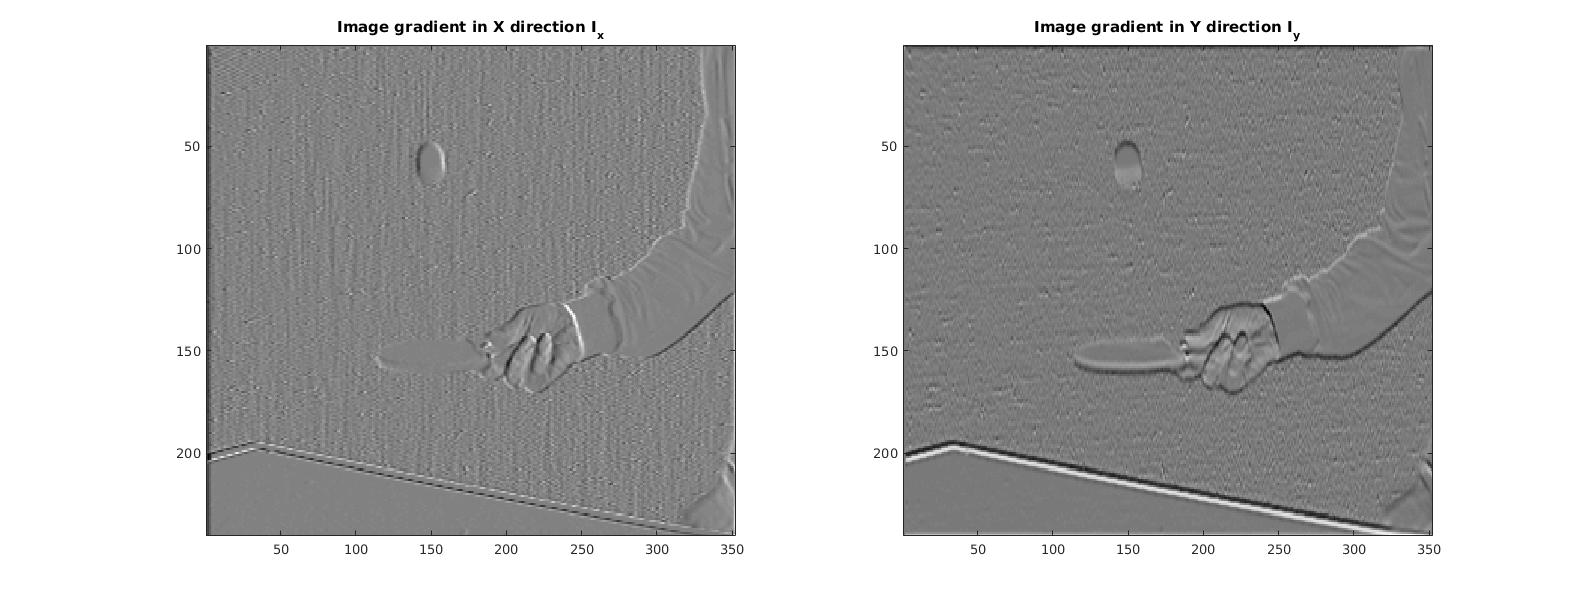
\includegraphics[width=1\textwidth]{imgs/derivatives_pingpong.jpg}
	\caption{Comparison for flowers.jpg. From left to right: original image, image
		filtered with 2D kernel and image filtered with 1D kernel. All images have a
		$\sigma$ value of 2}
	\label{fig:partialDerivatives_person}
\end{figure}



\section{Lucas-Kanade Algorithm for Optical Flow}



\section{Tracking}

\end{document}